% !TeX spellcheck = hu_HU
% !TeX encoding = UTF-8
% !TeX program = xelatex

\documentclass[11pt,a4paper,oneside]{report}             % Single-side
%\documentclass[11pt,a4paper,twoside,openright]{report}  % Duplex

% thanks to http://tex.stackexchange.com/a/47579/71109
\usepackage{ifxetex}
\usepackage{ifluatex}

\newif\ifxetexorluatex % a new conditional starts as false
\ifnum 0\ifxetex 1\fi\ifluatex 1\fi>0
   \xetexorluatextrue
\fi

\ifxetexorluatex
  \usepackage{fontspec}
  % xelatex-nél elég a fontspec include-olása
  % lásd: https://tex.stackexchange.com/questions/462664/warnings-when-using-babel-with-lualatex
  \def\magyarOptions{suggestions=no}
\else
  \usepackage[T1]{fontenc}
  \usepackage[utf8]{inputenc}
  \usepackage[lighttt]{lmodern}
\fi

\usepackage[magyar]{babel} % Alapértelmezés szerint utoljára definiált nyelv lesz aktív, de később külön beállítjuk az aktív nyelvet.

%\usepackage{cmap}
\usepackage{amsfonts,amsmath,amssymb} % Mathematical symbols.
%\usepackage[ruled,boxed,resetcount,linesnumbered]{algorithm2e} % For pseudocodes. % beware: this is not compatible with LuaLaTeX, see http://tex.stackexchange.com/questions/34814/lualatex-and-algorithm2e
\usepackage{booktabs} % For publication quality tables for LaTeX
\usepackage{graphicx}
\usepackage{subcaption}

%\usepackage{fancyhdr}
%\usepackage{lastpage}

\usepackage{anysize}
%\usepackage{sectsty}
\usepackage{setspace} % For setting line spacing

\usepackage[unicode]{hyperref} % For hyperlinks in the generated document.
\usepackage{xcolor}
\usepackage{listings} % For source code snippets.

% https://tex.stackexchange.com/a/224743
\lstset{
	basicstyle=\ttfamily,
	keepspaces=true,
	escapeinside={(*@}{@*)}, % only required for XeLaTeX
	columns=flexible, % only use with keepspaces=true       
	literate=*
	{á}{{\'a}}1
	{é}{{\'e}}1
	{í}{{\'i}}1
	{ó}{{\'o}}1
	{ö}{{\"o}}1
	{ő}{{\H{o}}}1
	{ú}{{\'u}}1
	{ü}{{\"u}}1
	{ű}{{\H{u}}}1
	{Á}{{\'A}}1
	{É}{{\'E}}1
	{Í}{{\'I}}1
	{Ó}{{\'O}}1
	{Ö}{{\"O}}1
	{Ő}{{\H{O}}}1
	{Ú}{{\'U}}1
	{Ü}{{\"U}}1
	{Ű}{{\H{U}}}1
}


\usepackage[amsmath,thmmarks]{ntheorem} % Theorem-like environments.

%\usepackage[hang]{caption}

\usepackage{array}
\usepackage{extdash}

\usepackage{tikz}
\usetikzlibrary{shadows}

% roviditesjegyzek
\usepackage[toc, acronyms]{glossaries}
\usepackage{makeidx}
\usepackage{tocbibind}

\makeglossaries
\makeindex


\singlespacing

\newcommand{\selecthungarian}{
	\selectlanguage{magyar}
	\setlength{\parindent}{2em}
	\setlength{\parskip}{0em}
	\frenchspacing
}

\newcommand{\selectenglish}{
	\selectlanguage{english}
	\setlength{\parindent}{0em}
	\setlength{\parskip}{0.5em}
	\nonfrenchspacing
	\renewcommand{\figureautorefname}{Figure}
	\renewcommand{\tableautorefname}{Table}
	\renewcommand{\partautorefname}{Part}
	\renewcommand{\chapterautorefname}{Chapter}
	\renewcommand{\sectionautorefname}{Section}
	\renewcommand{\subsectionautorefname}{Section}
	\renewcommand{\subsubsectionautorefname}{Section}
}

\usepackage[numbers]{natbib}
\usepackage{xspace}

\newcommand{\vikszerzoVezeteknev}{Főglein}
\newcommand{\vikszerzoKeresztnev}{Simon István}

\newcommand{\vikkonzulensAMegszolitas}{dr.~}
\newcommand{\vikkonzulensAVezeteknev}{Somogyi}
\newcommand{\vikkonzulensAKeresztnev}{Péter}

\newcommand{\vikkonzulensBMegszolitas}{}
\newcommand{\vikkonzulensBVezeteknev}{}
\newcommand{\vikkonzulensBKeresztnev}{}

\newcommand{\vikkonzulensCMegszolitas}{}
\newcommand{\vikkonzulensCVezeteknev}{}
\newcommand{\vikkonzulensCKeresztnev}{}

\newcommand{\vikcim}{Kiszolgálók üzemeltetése nagyvállalati környezetben és kapcsolódó szoftverek fejlesztése} % Cím
\newcommand{\viktanszek}{\bmeiit} % Tanszék
\newcommand{\vikdoktipus}{\bsc} % Dokumentum típusa (\bsc vagy \msc)
\newcommand{\vikmunkatipusat}{szakdolgozatot} % a "hallgató nyilatkozat" részhez: szakdolgozatot vagy diplomatervet

\input{include/tdk-variables}
\newcommand{\szerzoMeta}{\vikszerzoVezeteknev{} \vikszerzoKeresztnev} % egy szerző esetén
%\newcommand{\szerzoMeta}{\vikszerzoVezeteknev{} \vikszerzoKeresztnev, \tdkszerzoB} % két szerző esetén

% Beállítások magyar nyelvű dolgozathoz
\input{include/thesis-hu}
% Settings for English documents
%\input{include/thesis-en}

\input{include/preamble}

\linespread{1.5}

%--------------------------------------------------------------------------------------
% Table of contents and the main text
%--------------------------------------------------------------------------------------
\begin{document}

\pagenumbering{gobble}

\selectthesislanguage

%~~~~~~~~~~~~~~~~~~~~~~~~~~~~~~~~~~~~~~~~~~~~~~~~~~~~~~~~~~~~~~~~~~~~~~~~~~~~~~~~~~~~~~
\include{include/titlepage}		   % Szakdolgozat/Diplomaterv címlap
%\include{include/titlepage-tdk}	% TDK címlap
%\include{include/titlepage-otdk}   % OTDK címlap


% Table of Contents
%~~~~~~~~~~~~~~~~~~~~~~~~~~~~~~~~~~~~~~~~~~~~~~~~~~~~~~~~~~~~~~~~~~~~~~~~~~~~~~~~~~~~~~
\tableofcontents\vfill


% Declaration and Abstract
%~~~~~~~~~~~~~~~~~~~~~~~~~~~~~~~~~~~~~~~~~~~~~~~~~~~~~~~~~~~~~~~~~~~~~~~~~~~~~~~~~~~~~~
\include{include/declaration} %TODO Hallgatói nyilatkozat -- TDK és OTDK esetén törlendő!
\pagenumbering{roman}
\setcounter{page}{1}

\selecthungarian

%----------------------------------------------------------------------------
% Abstract in Hungarian
%----------------------------------------------------------------------------
\chapter*{Kivonat}\addcontentsline{toc}{chapter}{Kivonat}

Az informatika életünk szerves részévé vált: az interneten keresztül vásárolhatunk, intézhetjük banki ügyeinket és kommunikálhatunk egymással. Az egyre szélesebb körben elérhető szolgáltatások folyamatos üzemeltetése alapos tervezést, nagy szakértelmet és felkészültséget kíván meg a rendszermérnököktől.

A megnövekedett forgalom hatékony kiszolgálásához virtualizációs technológiákat alkalmaznak. Ezek lehetővé teszik, hogy számos különféle szolgáltatást tudjanak egy-egy szervergépen futtatni kedvező feltételek mellett: a virtualizáció csökkenti a szolgáltatások futtatásához szükséges helyigényt, és jobb erőforrás-kihasználtságot eredményez.

Az így létrejövő nagyméretű -- akár több ezer számítógépből álló -- infrastruktúrák karbantartása, üzemeltetése kézi megoldásokkal nehezen kivitelezhető. Emiatt jellemzően valamilyen infrastruktúra-menedzsment megoldást használnak a szervezetek, melyekkel központosítottan, egyetlen felületről van lehetőségük az üzemeltetett szerverek kezelésére, azok konfigurációjára.

A megfelelő minőségű üzemeltetéshez elengedhetetlen a számítógépek és az azokon futó szolgáltatások folyamatos felügyelete, monitorozása. Ennek segítségével figyelemmel követhetjük rendszereink állapotát, megfelelő határértékek beállításával pedig időben értesülhetünk az esetleges kialakulóban lévő problémákról, ezzel lehetőséget adva a hibák idejekorán történő javítására és a szolgáltatáskiesések megelőzésére.

Dolgozatomban a nagyvállalatokra jellemző informatikai környezeteket vizsgálom meg egy kis méretű tesztrendszeren keresztül. A tesztkörnyezetben kitérek a fent ismertetett technológiák alkalmazására, az ezek használata során követendő jó gyakorlatokra, és az általam tapasztalt kihívásokra, nehézségekre.


\vfill
\selectenglish


%----------------------------------------------------------------------------
% Abstract in English
%----------------------------------------------------------------------------
\chapter*{Abstract}\addcontentsline{toc}{chapter}{Abstract}

Information Technology (IT) has become an integral part of our lives, enabling us to shop, bank, and communicate online. The non-stop operation of an ever-wider range of services requires careful planning, expertise, and a high level of preparedness on the part of systems engineers.

Virtualisation technologies are used to efficiently serve the increased traffic. These allow a wide variety of services to run on a single server under favourable conditions: virtualisation reduces the space required to run services and results in better resource utilisation.

The resulting large-scale infrastructures -- up to thousands of computers -- are difficult to maintain and operate manually. For this reason, organisations typically use some kind of infrastructure management system that allows them to manage and configure the servers they operate from a centralised, single interface.

Continuous supervision and monitoring of computers and the services running on them is essential for ensuring the quality of operations. This allows us to monitor the status of our systems and, by setting appropriate thresholds, to be notified in time of any problems that may arise, thus providing the opportunity to correct errors in a timely manner and prevent service outages.

In my thesis, I examine IT environments typical of large enterprises through a small-scale test system. In the test environment, I will discuss the use of the technologies described above, the best practices to follow when using them, and the challenges and difficulties I have encountered throughout my work.


\vfill
\selectthesislanguage

\newcounter{romanPage}
\setcounter{romanPage}{\value{page}}
\stepcounter{romanPage}    %TODO Összefoglaló -- TDK és OTDK esetén nem kötelező


% The main part of the thesis
%~~~~~~~~~~~~~~~~~~~~~~~~~~~~~~~~~~~~~~~~~~~~~~~~~~~~~~~~~~~~~~~~~~~~~~~~~~~~~~~~~~~~~~
\pagenumbering{arabic}

%TODO import your own content
\newacronym{vm}{VM}{virtual~machine}
\newacronym{ha}{HA}{high~availability}
\newacronym{lvm}{LVM}{Logical Volume Manager}
\newacronym{pv}{PV}{physical volume}
\newacronym{vg}{VG}{volume group}
\newacronym{lv}{LV}{logical volume}

\newglossaryentry{hypervisor}
{
	name=hypervisor,
	description={Az a szoftver, amely koordinálja a virtuális gépek és az azokat futtató fizikai gép hardvere közötti interakciót}
}

\newglossaryentry{hotswap}
{
	name={hot swap},
	description={Számítógép-komponensek eltávolítása vagy hozzáadása egy futó rendszerhez (annak leállítása vagy újraindítása nélkül)}
}

% !TeX encoding = UTF-8
% !TeX spellcheck = hu_HU
%----------------------------------------------------------------------------
\chapter{\bevezetes}
%----------------------------------------------------------------------------

%A bevezető tartalmazza a diplomaterv-kiírás elemzését, történelmi előzményeit, a feladat indokoltságát (a motiváció leírását), az eddigi megoldásokat, és ennek tükrében a hallgató megoldásának összefoglalását.
%
%A bevezető szokás szerint a diplomaterv felépítésével záródik, azaz annak rövid leírásával, hogy melyik fejezet mivel foglalkozik.

Az informatika és az internet életünk szerves részévé vált. A számos szolgáltatás folyamatos rendelkezésre állásának biztosítása és a megnövekedett forgalom kiszolgálása jó néhány új technológia kifejlesztését követelte meg.

Dolgozatomban elsősorban egy általános képet szeretnék adni arról, hogy milyen üzemeltetési kihívásokkal kell szembenéznünk, ha ilyen szolgáltatásokat szeretnénk működtetni. Munkámban nem térek ki bizonyos infrastrukturális hátterekre -- mint például a~kiszolgálók folyamatos energiaellátásának biztosítása --, ezeket adottnak tekintem, hiszen ezt egy adatközpontban bérelt hely esetén sem magunknak kell biztosítanunk. A~következőkben sokkal inkább az informatikai lehetőségek tárgyalására helyezem a~hangsúlyt: hogyan tudunk hatékonyan üzemeltetni több kiszolgálót, milyen módon lehet biztosítani a szolgáltatásaink lehető legnagyobb rendelkezésre állását, és hogyan védhetjük meg adatainkat egy esetlegesen félresikerült rendszerfrissítést követően.

A dolgozatban érintem a jelenleg legelterjedtebb virtualizációs technológiákat, melyek főbb tulajdonságait röviden ismertetem, valamint össze is hasonlítom ezeket a~megoldásokat a legfontosabb különbségekre kitérve.

Szerepet kap továbbá a~logikai kötetkezelés, amely technológia nagyban megkönnyíti a~háttértárak és partíciók kezelését üzemeltetési szempontból. Ezt főként virtualizációt végző fizikai gépek esetében használhatjuk ki, hiszen ilyen helyzetekben érdemes minden virtuális rendszernek külön partíciót létrehozni, amelyek kezelése (pl.~egy esetleges bővítés során) a hagyományos particionálási megoldásokkal sokkal összetettebb feladat lenne. Dolgozatomban a Linux kernelben elérhető \acrfull{lvm} megoldást ismertetem részletesen. 

Szót ejtek a felügyeleti (monitoring) megoldásokról is, melyek elengedhetetlenek ahhoz, hogy a rendszer üzemeltetését végző szakemberek pontos képet kapjanak az infrastruktúra aktuális állapotáról, az esetleges korábbi problémákról. A monitorozás azért is fontos, mert ha egy hibát ezáltal sikerül idejekorán felismerni (például háttértárak esetén egy megfelelő határérték beállításával időben értesülhetünk egy partíció megteléséről, és~nem csak az írási hibákat tapasztaljuk), akkor elkerülhetőek a további, komolyabb hibák, amik akár a felhasználók számára is fennakadásokat okozhatnak. Az általam létrehozott tesztkörnyezetben is bemutatok egy ilyen monitoring megoldást, melynek segítségével a~munkám során kialakított infrastruktúra gépeit ellenőrzöm folyamatosan.

A tesztkörnyezet beállításában nagy szerep jut a~választott konfigurációmenedzsment szoftvernek, a~Salt-nak, mely egy~Python-alapú automatizációs eszköz informatikai rendszerek~kezelésére~\cite{SaltAbout}. Ez arra biztosít lehetőséget, hogy egyes konfigurációs \mbox{fájlokat} egyszerűen telepíthessünk több számítógépre is, valamint a keretrendszer leírónyelvén meghatározott konfiguráció-leíró szoftver lehetővé teszi szoftvercsomagok telepítését és a klienseken futó szolgáltatások (service) állapotának ellenőrzését is. Ez hasznunkra válhat például egy saját service-szel érkező program telepítését követően, hiszen így a leíróban megadhatjuk a telepítés paramétereit, majd ezt követően egyből ellenőrizhetjük is, hogy a telepítés után sikeresen elindult-e az újonnan telepített szoftver.


A dolgozatban tárgyalt koncepciókat egy kisebb volumenű tesztrendszeren keresztül mutatom be. Ennek a rendszernek a célja nem egy teljes vállalati környezet bemutatása, hiszen ehhez nagy mennyiségű hardverre, jelentős mértékű hardveres és szoftveres erőforrásokra lenne szükség, amelyek üzembe helyezése, összehangolása túlmutat a dolgozat keretein.
Ehelyett sokkal inkább arra szeretnék rávilágítani, hogy milyen eszközök állnak rendelkezésre egy ilyen nagyszabású infrastruktúra sikeres üzemeltetésének elősegítéséhez. Gondoljunk csak arra, hogy egy 5-10 számítógépből álló rendszer esetén kivitelezhető, hogy a rendszergazdák egyesével telepítsék a havi frissítéseket, azonban egy több száz, vagy több ezer kiszolgálóból álló nagyvállalati környezetben nem lenne reális elvárás.

Az ilyen és ehhez hasonló kihívások megoldására mutatok lehetőségeket  \aref{chap:technologies}.~fejezetben. Szó lesz a gépek távoli kezeléséről, folyamatos karbantartásukról, és biztonsági javításokról (patchek) való automatikus értesülésről. Tárgyalni fogom továbbá a rendszert alkotó eszközök monitorozását, metrikák gyűjtését, valamint szó lesz az egyre szélesebb körben elterjedő konténerizációs technológiákról. Bemutatom azt is, hogy a megfelelő eszközökkel milyen gyorsan hozhatunk létre konténereket, és milyen egyszerűen kezelhetjük őket akár egy böngészőből is.
Fontos megjegyezni, hogy az itt említett technológiák kisebb környezetekben is használhatóak, azonban néhány esetben az ilyen rendszerek használata kevesebb előnyt nyújt, mint amennyi munkát telepítésük és karbantartásuk igényel, így érdemes felmérni az~informatikai rendszerrel szemben támasztott elvárásainkat, és ennek megfelelően dönteni a szükséges technológiai komponensekről.

\Aref{chap:testenv}.~fejezetben ismertetem az általam készített tesztkörnyezet virtualizációs megoldását, ennek felépítését, komponenseit, a tervezési döntéseket, valamint az ezzel kapcsolatos munkáim során felmerült nehézségeket, tapasztalatokat. Ebben a fejezetben a korábban tárgyalt virtualizációs technológiák közül általam választott megoldás kezelését és néhány kapcsolódó jó gyakorlatot ismertetek.

A tesztkörnyezetben használt infrastruktúra-menedzsment megoldás konfigurációjáról és az ebben rejlő lehetőségekről \aref{chap:uyuni}.~fejezetben írok részletesen. Itt néhány példán keresztül bemutatom a konfigurációmenedzsmentben, csomagok telepítésében elérhető hatékony megoldásokat, kitérek a kliensek központi kezelésére. Emellett az~infrastruktúramenedzsment-szoftver használata során készített mérési eredményeimet is ismertetem.

Nagyvállalati, magas rendelkezésreállási követelményeket kielégíteni tudó rendszer lévén fontos kitérni az erőforrások, kiszolgálók folyamatos figyelésére, monitorozására. Az~erre kialakított monitoring rendszert \aref{chap:monitoring}.~fejezetben mutatom be részletekbe menően. Kitérek a környezet konfigurációjára, a probléma esetén küldésre kerülő riasztások beállítására, valamint a monitorozott rendszerekről gyűjtött adatok megjelenítésére.

Végül a dolgozat utolsó fejezetében értékelem az elért eredményeket, valamint röviden összefoglalom a projekt továbbfejlesztési lehetőségeit.



% !TeX encoding = UTF-8
% !TeX spellcheck = hu_HU

\chapter{Technológiai áttekintés}
\label{chap:technologies}

\section{Szervergépek}
\label{sect:servers}
A szerverek esetében jelentkező, egyénitől nagyban különböző felhasználási körülmények a szerverszámítógépek esetén hardveres szempontból is más felépítést igényelnek. A magas rendelkezésre-állás (\acrlong{ha}, \acrshort{ha}) és a modularitás, valamint az ezzel járó könnyű javítások támogatása érdekében az ilyen célra kialakított számítógépek főbb komponensei redundánsak, azaz egy-egy ilyen komponens kiesése nem jelent szolgáltatáskiesést. A meghibásodást a rendszer egyértelműen jelzi magán a gépházon is (általában hibajelző LED-ek segítségével), valamint a menedzsment portjain is. A legtöbb ilyen gép ugyanis rendelkezik egy beágyazott rendszerrel, ami lehetővé teszi a távoli kezelésüket egy webes felületen és SSH-n keresztül még akkor is, ha a szervergép ki van kapcsolva. Ezek lehetőséget biztosítanak a gép legfontosabb mérőszámainak követésére, virtuális kijelző csatlakoztatására, telepítőfájlok felcsatolására, valamint a gép ki- és bekapcsolására.

\begin{figure}[!ht]
	\centering
	\includegraphics[width=150mm, keepaspectratio]{figures/ilo-power1.png}
	\caption{Szervergép fogyasztásának grafikonja egy HPE számítógép távoli menedzsment felületén. Vegyük észre a jobb alsó sarokban megjelenő menüt, amivel lehetőségünk van a gép kikapcsolására és újraindítására is.}
	\label{fig:ilopowerchart}
\end{figure}

A fent ismertetett üzemeltetést, karbantartást könnyítő felépítés mellett általában elmondható, hogy az ilyen gépek jelentős része virtualizációra van tervezve -- persze ezektől különböző felhasználási módok is jelentkeznek (például fájlszerverek tervezése során a teljesítmény helyett a minél nagyobb tárkapacitásra és adatátvitelre helyezték a hangsúlyt). A dolgozat szempontjából viszont a nagyvállalati környezetben domináló virtualizációs felhasználási terület lesz a lényegesebb, így a továbbiakban az ilyen számítógépekre fogok koncentrálni.

A virtualizációs hosztgépek jellemzője, hogy számos processzorral rendelkeznek, valamint felhasználói szemmel szokatlanul nagy memóriaterülettel bírnak. Ki fog derülni azonban, hogy 12-24 processzormag és akár több száz gigabyte RAM is szűkös erőforrássá válhat egy virtuális gépeket futtató számítógép esetében, hiszen gyakorlatilag itt egyetlen szervernek kell elbírnia akár több tíz számítógép terhelésével is. Ezek mellett általában több (8-24) háttértár-foglalattal is rendelkeznek, melyekhez hardveres RAID-támogatást is adnak.
% TODO: kép a gépről

\section{Virtualizáció}
A fent említett megnövekedett forgalom kiszolgálását hatékonyan lehet kezelni úgy, hogy olyan fizikai számítógépet helyezünk üzembe, mely  több, egymástól független operációs rendszer futtatására is alkalmas. Ilyenkor ezeket a fizikai gépen futó rendszereket virtuális gépeknek (\acrlong{vm}, \acrshort{vm}) nevezzük. Egy virtuális gép elkülönített erőforrásokat kap a fizikai géptől, hozzáférhet például bizonyos mennyiségű processzormaghoz, memóriához, illetve külön háttértár-partíciói is lehetnek. A virtualizált hardverek és operációs rendszerek a legtöbb esetben a külvilág felé nem különböztethetőek meg a fizikai számítógépektől, és ezzel a megoldással jelentősen csökkenthető a rendszerek és a hozzájuk szükséges informatikai infrastruktúra üzemeltetésének költsége.

A virtualizáció nagy ereje abban rejlik, hogy bizonyos hardverek virtualizációjával egységnyi teljesítményt olcsóbban kaphatunk meg, mintha külön fizikai gépeket helyeznénk üzembe, illetve nagyobb rugalmasságot kapunk a kezelésükben, üzemeltetésükben. Képzeljük el, hogy megveszünk egy számítógépet, amin szeretnénk futtatni egy számunkra fontos alkalmazást, mondjuk a honlapunkat. Ilyenkor az ezen a gépen futó operációs rendszer teljes mértékben megszabhatja, hogy milyen erőforrásokból mennyit használ. Ha egy másik szolgáltatást -- például levelezőszervert -- szeretnénk emellett futtatni, akkor limitáltabbak a lehetőségeink, hiszen a korábban telepített webszerver már foglal bizonyos erőforrásokat, illetve a program függőségeit és konfigurációs fájljait is telepítettük már, ami esetleg negatívan hat a levelezőszerverünk működésére. Ha mindezt virtualizált környezetben tesszük meg, akkor a topológia megváltozik: a két alkalmazás teljesen elkülönítetten, egymás zavarása nélkül, különböző virtuális gépekben futhatnak, ezeket a gépeket pedig a fizikai gépen futó egyik szoftverkomponens, az úgynevezett \gls{hypervisor} kezeli, mely a gazdagépen futó rendszer legfőbb virtualizációt támogató komponense~\cite{Sles15virt}. A \gls{hypervisor} látja el az erőforrások ütemezésének és kiosztásának (pl.~processzoridő, memória) feladatát, gondoskodik a virtuális gépek számára szükséges hardveres erőforrások virtualizált hardverinterfészeken keresztüli elérhetőségéről.
% TODO: virt-manager screenshot, esetleg virsh xml screenshot

\subsection{Népszerű virtualizációs technológiák}
Mivel a virtualizáció napjainkban nagyon elterjedt technológia, számos olyan megoldás született, mely egyszerűsíti a virtuális gépek üzemeltetését. Ezek közül nagy ismertségnek örvend az Oracle~VirtualBox és a VMware~Player, azonban ezek a megoldások nem skálázódnak annyira jól, mint a továbbiakban tárgyalt társaik, melyek sokkal megfelelőbbek nagyvállalati szerverkörnyezetben való alkalmazásra. Ezek a \gls{hypervisor}ok lehetőséget biztosítanak a virtuális gépek távoli elérésre, kezelésére, egyszerűbb telepítésükre, valamint szükség esetén elosztott működésükre. A következőkben három népszerű virtualizációs technológiát fogok bemutatni, összehasonlításuk \aref{tab:hypervisor-comparison}.~táblázaton látható.

A \gls{hypervisor}okat két kategóriába sorolhatjuk Robert P. Goldberg 1973-as publikációja alapján~\cite{Goldberg1973Hypervisors}. Az egyes típusú hypervisorok \mbox{(type-1)} natívan, közvetlenül a gazdagépen futnak (pl.~a következőkben tárgyalt VMware~ESXi), míg a kettes típusba tartozó \mbox{(type-2)}, úgynevezett hosztolt hypervisorok egy hagyományos operációs rendszeren futnak más számítógépes programokhoz hasonlóan. Kettes típusú hypervisor például az Oracle~\mbox{VirtualBox}. Egyes hypervisorok --~mint a~\acrshort{kvm}~-- besorolása vitatott, mivel egy kernelmodulként épül bele egy már futó \acrshort{os}-be. Azonban mivel azt így lényegében egy type-1 \gls{hypervisor}rá alakítja, ezért általában az egyes típusba sorolják~\cite{WikiHypervisor}. A két típus felépítését \aref{fig:hypervisors}.~ábra mutatja be.

\begin{figure}[ht]
	\centering
	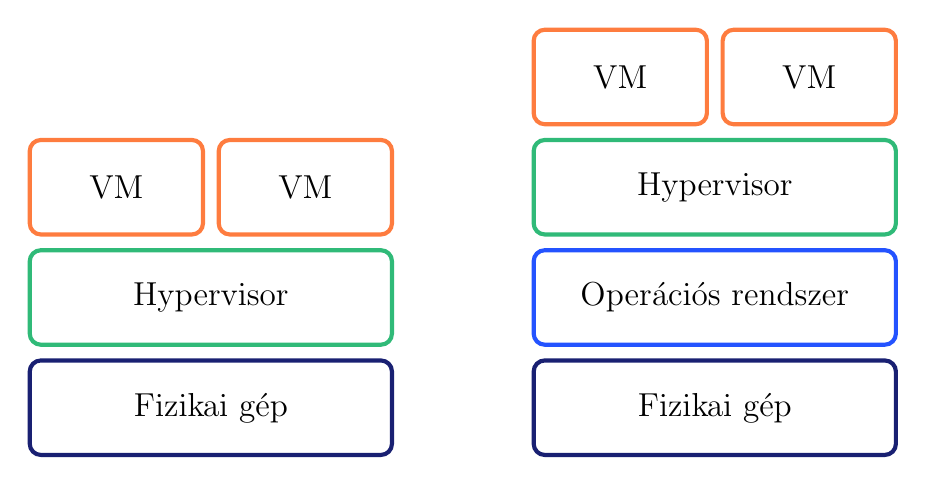
\begin{tikzpicture}[node distance=1.4cm]
	\definecolor{midnightblue}{HTML}{192072}
	\definecolor{junglegreen}{HTML}{30BA78}
	\definecolor{waterholeblue}{HTML}{2453FF}
	\definecolor{persimmon}{HTML}{FE7C3F}

	\tikzstyle{rect} = [rectangle, rounded corners, draw=midnightblue, minimum width=4.6cm, minimum height=1.2cm, text centered, text=black, font=\fontsize{12}{12}\selectfont, line width=1.5pt]
	\tikzstyle{vm-rect} = [rectangle, rounded corners, draw, minimum width= 2.2cm, minimum height=1.2cm, text centered, font=\fontsize{12}{12}\selectfont, line width=1.5pt]
	
	\node (hardware) [rect] {Fizikai gép};
	\node (hypervisor) [rect, above of = hardware, draw=junglegreen] {Hypervisor};
	\node (vm1) [vm-rect, above of = hypervisor, xshift=-1.2cm, draw=persimmon] {VM};
	\node (vm2) [vm-rect, above of = hypervisor, xshift=1.2cm, draw=persimmon] {VM};

	\node (hardware2) [rect, right of = hardware, xshift=5cm] {Fizikai gép};
	\node (os) [rect, above of = hardware2, draw=waterholeblue] {Operációs rendszer};
	\node (hypervisor2) [rect, above of = os, draw=junglegreen] {Hypervisor};
	\node (vm1_2) [vm-rect, above of = hypervisor2, xshift=-1.2cm, draw=persimmon] {VM};
	\node (vm2_2) [vm-rect, above of = hypervisor2, xshift=1.2cm, draw=persimmon] {VM};

\end{tikzpicture}

	\caption{Type-1 és type-2 \gls{hypervisor}ok felépítése.}
	\label{fig:hypervisors}
\end{figure}

Nagyvállalati környezetben elterjedt virtualizációs megoldás például a VMware~ESXi, amely egy igen modern \gls{hypervisor} számos kényelmi funkcióval ellátva (lehetőség van például a rendszer webes felületről való kezelésére és virtuális gépek sablonból való gyors, körülbelül 5-10 perc alatti telepítésére). Az ESXi a részletes beállításokat lehetővé tevő, könnyen kezelhető webes felületének köszönhetően nagy piaci részesedést szerzett, felmérések alapján kb. 60-80\%-os jelenléttel uralja a virtualizációs piacot, bár a közelmúltban bevezetett új, jelentősen drágább előfizetési modell némileg csökkenthet ezen az arányon~\cite{VmwareMarketshare}~\cite{VmwareCustomerDecline}.
Egy másik kedvelt megoldás az ESXi-vel ellentétben felhasználási korlátozás nélkül teljesen ingyenesen, GPLv2-es licenc alatt elérhető XEN~\gls{hypervisor}. Ez ugyan kevesebb kényelmi funkciót tartalmaz, de szintén népszerűségnek örvend széleskörű támogatása, kedvező teljesítménye és szabad szoftver voltából eredő ingyenessége miatt. A XEN a 2014~márciusában kiadott 4.4-es~verzió óta stabilan működik együtt a \gls{libvirt} virtualizációs \acrshort{api}-val, amely nagyban megkönnyíti a \gls{hypervisor}ral való kommunikációt a virtuális gépek konfigurálása során~\cite{Xen44ReleaseNotes}.

A XEN-hez hasonlóan szabad szoftver licenccel érhető el a \acrfull{kvm} is, mely a XEN-nél modernebb megoldásnak tekinthető, és manapság széles körben használják a Linux kernelbe való integráltságának és stabilitásának köszönhetően. Bár maga a \acrshort{kvm} nem tartalmaz ilyet, de számos interfész elérhető az ezen keresztül futtatott virtuális gépek kezelésére (például~virt-manager és további, a XEN-nél említett \gls{libvirt} \acrshort{api}-t támogató  szoftverek), valamint akadnak olyan megoldások is, melyek a \acrshort{kvm}-re alapozva nyújtanak szélesebb körű virtualizációs megoldást, ilyen lehet\footnote{A konfigurációtól függően akár többfajta virtualizációs környezet is beállítható, de a \acrshort{kvm} az egyik legjobban támogatott.} például a Proxmox és a Cockpit.

\begin{table}[h!]
	\setlength{\tabcolsep}{5pt}
	\renewcommand{\arraystretch}{1.3}
	\centering
	\begin{tabular}{||p{3.25cm} p{3.25cm} p{3.25cm} p{3.25cm} ||}
		\hline
		Megnevezés & VMware ESXi & XEN & KVM \\
		\hline\hline
		Fejlesztő & VMware LLC & Linux Foundation, Intel & Linux fejlesztői közösség \\
		\hline
		Licencelés & zárt forráskódú, korlátozott ingyenes verzió, teljes verzióhoz előfizetés szükséges & szabadon hozzáférhető, GPL & szabadon hozzáférhető, GPL \\
		\hline
		Támogatott architektúrák & x86-64, ARM & IA-32, x86-64, ARM & ARM, PowerPC, ESA/390, IA-32, x86-64 \\
		\hline
		\Gls{hypervisor} típusa & Type-1 & Type-1 & Type-1 \\
		\hline
		Hivatalosan támogatott \acrshort{vm} \acrshort{os}-ek & Linux, BSD, Windows, macOS & Linux, BSD, Windows, macOS & Linux, BSD, Windows, macOS \\
		\hline
		Aktív \gls{libvirt} támogatottság & Limitált & Igen & Igen \\
		\hline
		Támogatás & Hivatalos & Közösségi & Közösségi  \\
		\hline
		\acrshort{cpu} hot swap & Igen & Igen & Igen \\
		\hline
		Memória hot swap & Igen & Igen & Igen \\
		\hline
		Megjegyzés & Könnyű kezelhetőségének, jó támogatásának köszönhetően napjaink legelterjedtebb virtualizációs platformja. & Eredetileg egyetemi projektként indult, a 2000-es évek közepén nagy fejlődésen ment keresztül, számos nagy platform (pl.~Amazon~AWS) építi XEN-re a virtualizációs technológiáját. & Hivatalosan is a Linux kernel része, így folyamatos fejlesztés alatt áll és hatékonyan együtt tud működni a kernellel. Számos virtualizációs platform (pl.~Google Cloud Platform) alapjaként szolgál.  \\
		\hline
	\end{tabular}
	\caption{A tárgyalt virtualizációs megoldások összehasonlítása.}
	\label{tab:hypervisor-comparison}
\end{table}


\subsection{Virtuális gépek használatának néhány előnye}
A virtualizáció számos előnnyel járhat az infrastruktúra és a kiszolgálni kívánt alkalmazások szempontjából. Az egyik legnagyobb ilyen előny például, hogy a virtuális gépek egymástól izoláltan futnak, azaz nincs közvetlen kapcsolat közöttük, ami biztonsági és kezelési, tesztelési szempontból is kedvező lehet. Egy adott csomag vagy szoftver kipróbálásához például készíthetünk egy teszt virtuális gépet, amit egyszerűen törölhetünk a teszt végeztével --~a telepített program eltávolítása hagyományos környezetben futtatva sokkal körülményesebb lenne. Hasonlóan előnyökkel jár, hogy a legtöbb modern \gls{hypervisor} lehetőséget biztosít bizonyos erőforrások úgynevezett \gls{hotswap}-elésére. Ez azt jelenti, hogy egyes komponenseket (pl. memória) úgy is bővíthetünk, hogy a rendszert nem szükséges ehhez leállítanunk.
A felsoroltak mellett néhány további előnyt szeretnék részletesen ismertetni a következő alfejezetben.

\subsubsection{Erőforrások testreszabása}
Amikor több tíz vagy több száz szerver üzemeltetéséről van szó, akkor hatványozottan számításba kell vennünk az egyes gépekre jutó költségeket. Virtuális gépek esetén ez azért kedvezőbb egy fizikai gépnél, mert ugyan a nagyvállalati környezetbe szánt szervergépek jelentősen drágábbak a személyes felhasználásra tervezett társaiknál, de akár több tíz virtuális gép egyidejű futtatását is lehetővé teszik. Ezáltal az egy fizikai gépre eső, asztali gépeknél megszokott áramfogyasztáshoz képest jóval nagyobb energiafelvétel sokkal kedvezőbb arányt mutat, ha számításba vesszük a futtatott virtuális kiszolgálók számát is.

Mindezek mellett a nagyvállalati felhasználáshoz tervezett számítógépek jóval hibatűrőbbek, hiszen a főbb komponensek redundánsan lettek kialakítva: ezekből az ilyen szerverekben legalább kettő van, és a rendszer automatikusan képes detektálni a hardveres hibákat, és ezek figyelembe vételével tovább működni. További előny lehet még hardveres hibák esetén, hogy ezek a számítógépek széles körben támogatják az úgynevezett \textit{hot swappingot}, amely azt jelenti, hogy bizonyos hardverelemek (általában például háttértárak és memóriamodulok) a számítógép bekapcsolt állapotában, annak működése közben is szolgáltatás nélkül cserélhetőek.

Előnyös lehet továbbá, hogy a virtuális gépek erőforrásai szabadon módosíthatók, így akár két újraindítás között is változtathatjuk a rendelkezésre álló memória mennyiségét vagy épp a processzormagok számát. Sőt, egyes hypervisorok és operációs rendszerek ezen erőforrások futásidejű megváltoztatását is támogatják bizonyos korlátozások mellett, így gyakorlatilag a fontosabb virtualizált erőforrások is hot swappelhetőnek tekinthetőek.

\subsubsection{Snapshotok}
Egy másik kedvező lehetőség virtuális gépek használata esetén az, hogy úgynevezett snapshotokat készíthetünk róluk. Ezek a snapshotok a gépet egy adott pillanatbeli állapotban reprezentálják, és később ezeket az állapotokat visszaállíthatjuk, ha szükségünk lesz rá. Egyes megoldások a memóriakép mentését is támogatják, így akár egy futó gép is könnyen visszaállítható. A snapshotok készítése hasznos lehet például rendszerfrissítések esetén, így ha valamiféle hiba lép fel a frissítés során, vagy egy adott szoftver nem megfelelően működik azt követően, akkor a frissítés előtt készített snapshotra visszaállva újra teljes értékűen üzemelhet a szerver, amíg a frissítés során fellépő hibát elhárítjuk.

\subsubsection{Migráció}
Részben az előző ponthoz kapcsolódik a virtuális gépek migrációja. Ez a funkció azt jelenti, hogy egy adott fizikai gépről, mely virtuális gépeket futtat (virtual host), készíthetünk egy snapshotot, amit áthelyezhetünk egy másik virtual hostra, és a virtuális gép ezen futhat tovább egyéb újrakonfigurálás nélkül.
Lehetőség van azonban a háttértárak tartalmát elhagyva is átmozgatni egy VM-et egy másik hosztra. Ehhez bevett szokás leírófájlok használata, mely egy virtuális gép konfigurációját tartalmazza. A leírófájlt egy másik hosztgépre áthelyezve ott újra elindíthatjuk a definiált virtuális gépet. Ilyenkor szükség lehet a VM háttértárainak inicializálására, de ettől eltekintve a konfiguráció szabadon hordozható virtual host-ok között. Ilyen migrációra egyes megoldások fejlettebb támogatást is adnak, így akár valós időben, az aktuális terheltség figyelembe vétele mellett automatikusan is áthelyezhetőek virtuális gépek a megadott fizikai hosztok között.
% TODO: listing egy példa virsh xml-lel

\subsection{Konténerizáció}


\section{RAID}
Nagyvállalati környezetben nem hagyhatjuk ki a RAID-megoldásokat (a népszerű RAID~1-et és RAID~6-ot \aref{fig:raid}.~ábra szemlélteti), ha adatok biztonsági mentéséről beszélünk. Ezek arra adnak lehetőséget, hogy az adatokat több háttértáron (pl. merevlemez vagy SSD) tároljuk úgy, hogy egy esetleges diszk hiba ne okozzon fennakadást a működésben. Fontos tisztában lenni azonban azzal, hogy a RAID-megoldások nem védenek bizonyos veszélyek ellen (például zsarolóvírusok, fájlok korruptálódása), hiszen az adatok duplikálása valós időben történik, így egy esetleges támadás során a RAID pool-ba bevont összes diszken megváltoznak az adatok, így nem alkalmas a támadás utáni visszaállításra. Emiatt egy RAID pool a \textit{3-2-1} mentési stratégiát alkalmazva csak egyetlen eszköznek tekinthető, hiába több lemezt használunk a mentés során. RAID-elést tehát csak hardveres hibák ellen érdemes használnunk, rosszindulatú támadás esetén ezek nem nyújtanak védelmet az adataink számára.

% TODO: RAID ábra, hivatkozások
\begin{figure}[!ht]
	\centering
	\begin{subfigure}{0.3\textwidth}
		\centering
		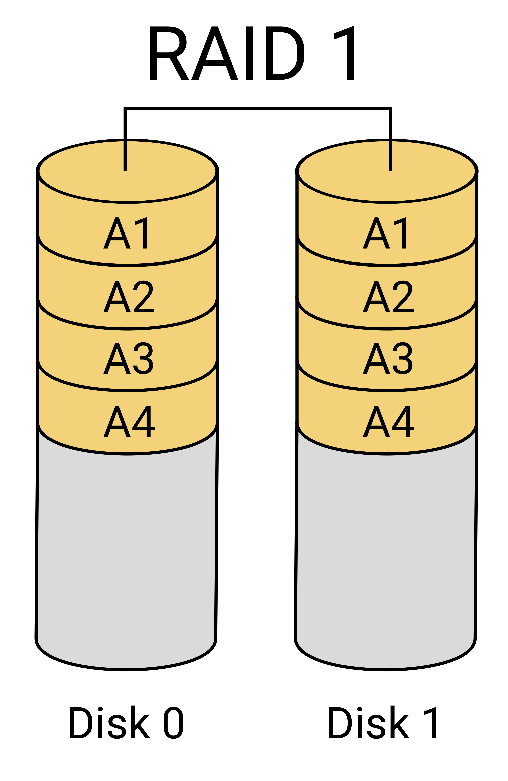
\includegraphics[keepaspectratio, height=52mm]{figures/raid1.pdf}
	\end{subfigure}
	\hspace{0.05\textwidth}
	\begin{subfigure}{0.6\textwidth}
		\centering
		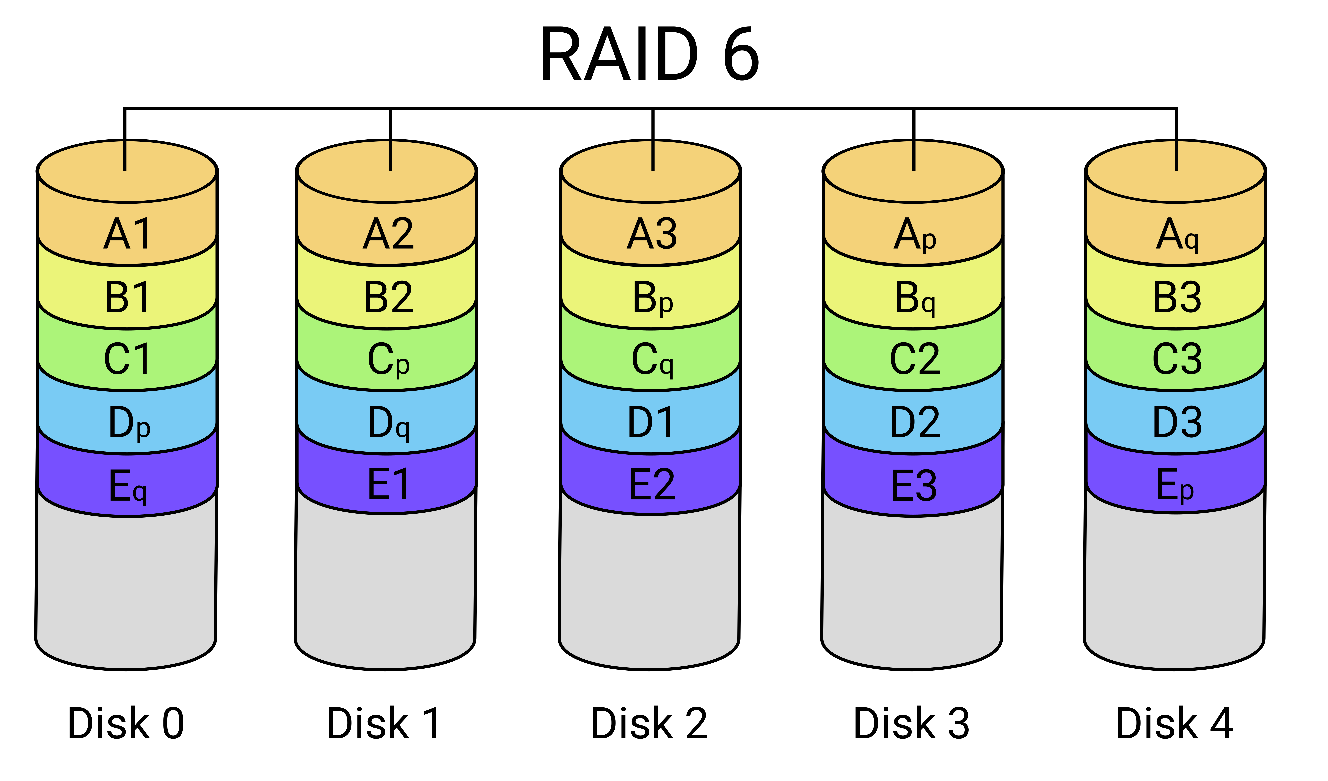
\includegraphics[keepaspectratio, height=52mm]{figures/raid6.pdf}
	\end{subfigure}
	\caption{RAID 1 és RAID 6 megoldások felépítése \cite{WikiRaidLevels}}
	\label{fig:raid}
\end{figure}


\section{Logikai kötetkezelés}
\label{sect:lvm}
Mind a fizikai, mind a virtuális gépek esetén szükség lehet háttértárakra az adatok perzisztens tárolása érdekében. Hagyományos particionálási megoldásokkal hamar nehezen kezelhetővé válhatnak a különböző csatolási pontok és a virtuális gépek számára kiosztott kötetek. Az ilyen problémák elkerülésére jött létre a logikai kötetkezelés, mely a tárhely-virtualizáció egy formája. A logikai kötetkezelésnek több implementációja létezik. % TODO: cite wikipedia: https://en.wikipedia.org/wiki/Logical_volume_management
Ezek közül jelenleg a Linux kernelben elérhető \gls{lvm}-et fogom részletesen ismertetni.

A Linux logikai kötetkezelője három lényegi rétegből áll: a fizikai kötetből (physical volume, PV), a kötetcsoportból (volume group, VG) és a logikai kötetekből (logical volume, LV). Ezt a felépítést \aref{fig:lvm} ábra szemlélteti egy egyszerű \gls{lvm}-konfiguráción keresztül.
Lehetőség van ennél összetettebb kötetkiosztás létrehozására is, például egy kötetcsoport több fizikai kötetből is állhat, amik akár külön háttértáron is lehetnek, sőt, RAID-csoportot is megadhatunk egy \gls{lvm}-partíció alapjául. Ezen megoldások használata azonban sok hátránnyal járhat (pl. diszkhiba esetén nehezebb visszaállítani a partíciót), ezért ennek használata alapvetően nem ajánlott~\cite{RHLVM}.

Az \gls{lvm} tehát úgy épül fel, hogy egy vagy több háttértáron létrehozunk hagyományos fizikai partíciókat, melyek az \gls{lvm} \acrshort{pv}-k alapjául fognak szolgálni. Ezt követően létrehozzuk a kötetcsoportokat az általuk használandó \acrshort{lvm} fizikai kötetek megadásával. Az így létrejött csoportban már tudunk létrehozni logikai köteteket, amíg van szabad hely a \acrshort{vg}-ben.

Láthatjuk, hogy az \acrshort{lvm}-kötetek használata kezdetben több feladattal jár, mint a hagyományos partíciók esetében, azonban hosszabb távon számos előnnyel jár. Talán a logikai kötetkezelés legnagyobb előnye, hogy szabadon allokálhatunk tárterületet a létrehozott köteteknek: ha azt tapasztaljuk, hogy az egyik köteten kevés a szabad hely, akkor fájlrendszertől függően elég lehet akár egy parancs kiadása is ennek kiterjesztéséhez. Lényeges, hogy a hagyományos partíciók használatával ellentétben a logikai kötetkezelés használatakor figyelmen kívül hagyhatjuk a partíciók elhelyezkedésének sorrendjét, így nem szükséges figyelembe vennünk, hogy az adott partíció előtt vagy után van-e szabad tárterület. A megnövelt kötet helyes fizikai háttértárra képzéséről a logikai kötetkezelő fog gondoskodni számunkra. Fontos megjegyezni, hogy a kötetbővítés online is elvégezhető, azaz nem szükséges a kötetet lecsatolni a gépről az átméretezéshez. Ez különösen fontos lehet például a root~(/) partíció növelése során, hiszen ezt csak a számítógép leállítása mellett tudjuk biztonságosan lecsatolni. Előállhat olyan helyzet is, hogy egy másik (nem root) partíciót kell online átméreteznünk, például ha azt tapasztaljuk, hogy egy adatbázisszerveren hirtelen nagy mértékben nőtt a tárolt adat mérete. Ilyenkor nincs lehetőség a szerver leállítására, hiszen ez esetben az alkalmazások nem tudnák használni az adatbázist a leállás idejére. Az ehhez hasonló helyzetekre is jó megoldást nyújt a logikai kötetkezelő egy megfelelő, online átméretezést támogató fájlrendszer (pl. XFS, Btrfs) használata mellett. Érdemes megjegyezni, hogy bár az \acrshort{lvm} és például a Btrfs-fájlrendszer nyújt támogatást a növelésen kívül a fájlrendszer méretének csökkentésére is, ez a művelet általában nem biztonságos, és adatvesztéshez vezethet. Emiatt érdemes eleinte csak kisebb tárterületet adni a köteteinknek, hiszen kiterjeszteni sokkal egyszerűbb őket, mint csökkenteni a méretüket. Ennek megkönnyítésére is ad lehetőséget az \acrshort{lvm}, megadhatjuk, hogy egy kötet egy bizonyos arányú tárhelyhasználat után automatikusan bővüljön, így elkerülve annak betelését.

Az \acrshort{lvm} hasznos funkciói közé tartozik még a kötetpillanatképek (volume snapshots) készítésének lehetősége. Ez azt jelenti, hogy a kötetkezelő képes az adott kötet adott pillanatbeli helyzetének rögzítésére, és erre a verzióra szükség szerint visszaállhatunk (rollback). Ez hasznos lehet például nagyobb konfigurációs változások eszközölése esetén, gyorsan változó adatokkal dolgozó rendszerek (pl. adatbázisszerver) biztonsági mentéseinek készítése során, illetve rendszerfrissítések előtt.\footnote{Egyes eszközök és operációs rendszerek (pl. openSUSE-verziók a snapper-rel (\url{https://doc.opensuse.org/documentation/leap/reference/html/book-reference/cha-snapper.html}) automatikusan készítenek snapshotot a frissítések telepítése előtt, így hiba esetén visszaállhatunk a frissítés előtti verzióra.}



\begin{figure}[!ht]
	\centering
	\includegraphics[width=14cm]{figures/lvm.pdf}
	\caption{Egyszerű \acrshort{lvm}-kötetkezelési hierarchia.}
	\label{fig:lvm}
\end{figure}

\section{OS-lehetőségek} \label{sect:os}
Egy nagyvállalati informatikai infrastruktúrában nagy szerepe van a választott operációs rendszernek is, ugyanis nem mindegy, hogy a több száz számítógépből álló rendszerünket mennyire hatékonyan tudjuk karban tartani, egy kritikus biztonsági frissítést milyen hamar tudunk telepíteni az érintett eszközökre, és probléma vagy különleges igény esetén milyen támogatásra számíthatunk a szoftvereinket illetően.
Ezeket a szempontokat figyelembe véve manapság elsősorban a Debian, Ubuntu, Red Hat Enterprise Linux és SUSE Linux Enterprise diszribúciók közül választanak a vállalatok.

A Debian stabilitása miatt népszerű választás elsősorban kisebb (néhány tíz gépből álló) infrastruktúrák esetében, viszont a stabilitás az elérhető csomagok verzióinak rovására megy, általában a legújabbnál néhány verzióval régebbi csomagokat szállítanak a disztribúcióval. A Debian előnye, hogy teljesen ingyenesen elérhető, és bár nincs hozzá hivatalos támogatás, harmadik féltől vásárolhatunk ilyen szolgáltatást.

Az Ubuntu egy Debian-alapú operációs rendszer, melyet a Canonical Ltd. fejleszt, és vállalati támogatást is nyújt az OS-hez amellett, hogy az alapverzió ingyenesen érhető el. Előnye, hogy mivel mind szerver, mind pedig asztali környezetben elterjedt rendszer, számtalan projekt és gyártó adja ki a szoftvereit Ubuntu rendszerekre.

A Red Hat és a SUSE Linux-verziók már inkább egy magasabb kategóriát céloznak meg: fő célközönségük a több száz, illetve több ezer gépes környezetet üzemeltető vállalatok, és a fent említett két disztribúciónál alapesetben (a legkisebb támogatási csomagban) is szélesebb körű támogatást biztosítanak az operációs rendszerekhez. Kiemelendő, hogy ez a két disztribúció egyedülálló a biztonság területén: számos biztonsági tesztnek vetették alá őket különböző szervezetek (köztük például kormányzatok és IT-biztonságra specializálódott cégek is), melyeket követően a kereskedelmi forgalomban lévő Linux-disztribúciók közül a legmagasabb minősítéseket és tanúsítványokat kapták meg ezek a rendszerek~\cite{RhSec}~\cite{SlesSec}.

Lényeges különbség még, hogy az utóbbi két operációs rendszer \acrshort{rpm}-alapú csomagkezelőt használ, mely a Debian és Ubuntu által használt DEB formátumhoz képest több lehetőséget biztosít például javítások (patchek) telepítésére. Emellett ez a formátum általában jobb támogatottságot élvez vállalati szoftverek esetében, ezért ezekben a felhasználási körökben az \acrshort{rpm}-csomagokat használnak a DEB-csomagokkal szemben.


\section{Infrastruktúramenedzsment}
Komplex infrastruktúrák esetén egyre nehezebbé válik a szerverek konfigurációjainak karbantartása, a frissítések kezelése. Manapság már széles körben elterjedtek az infrastruktúramenedzsment-megoldások, melyek lehetőséget biztosítanak ezen problémák kiküszöbölésére. Alkalmazásukkal hatékonyabbá tehető a számítógépek szoftveres karbantartása, könnyen egységesíthetőek a konfigurációs állományok, és így egyszerűbben kezelhetővé válnak az azonos szerepű számítógépek, rendszercsoportok.

\subsection{Ansible és Salt}
Dolgozatomhoz az Ansible-t és az Uyuni alapjául szolgáló Salt-ot vizsgáltam meg közelebbről. Mindkét megoldás elterjedtnek tekinthető, azonban a felépítésük nagyban különbözik.

Az Ansible sikere az egyszerűségében rejlik: az Ansible szerveren, az úgynevezett \textit{Control Node}-on kívül nincs szükség további komponensek telepítésére az alapvető funkciók használatához. Az Ansible nem használ dedikált kliensszoftvereket, ezért \textit{agentless}-nek nevezik, működése a push modellen alapul. A feladatok végrehajtását, konfigurációs fájlok elhelyezését úgynevezett Playbook-okkal adhatjuk meg, melyek YAML-ben írt leírófájlok. Egy-egy ilyen fájl több, egymástól független, tetszőleges komplexitású feladatot definiálhat. A \textit{Control Node} ezeket \acrshort{ssh}-n keresztül hajtja végre, ehhez a kliensek \acrshort{ssh}-kulcsát kell megadnunk. A megoldás előnye, hogy így az autentikáció és a kommunikáció titkosságának fenntartása is jelentősen egyszerűsödik, hiszen egy már jól bevált, biztonságos komponensen alapul~\cite{RedHatAnsibleVsSalt}.

Az Ansible-lel szemben a Saltot a kezelt rendszerekre is szükséges telepíteni. A Salt felépítése két kulcsfontosságú komponensre osztható: a Salt Masterre és a Salt Minionokra (emiatt \textit{agent-based} architektúrának nevezik). Minionoknak a kliensekre telepített komponenst nevezzük, mely a későbbiekben az úgynevezett Salt State-ekben meghatározott feladatok végrehajtásáért lesz felelős, melyeket a Master delegál ki a kliensek számára. A feladatleírók, a State-ek a Salt esetében is YAML-alapúak. A Salt architektúrájában a kezdeti kapcsolatfelvételt a minion indítja a publikus RSA-kulcsának elküldésével, ezt manuálisan kell ellenőrizni és elfogadni a Masteren. Ha a kulcs elfogadásra kerül, a szerver is elküldi a saját publikus kulcsát a Minionnak~\cite{SaltSecurity}. Ezt követően a Salt Master már képes a bevont Minionnak végrehajtandó feladatokat küldeni, valamint a Minion állapotát lekérdezni~\cite{RedHatAnsibleVsSalt}.

\section{Monitoring}
\label{sect:monitoring}
Informatikai környezet üzemeltetése során fontos valós időben tisztában lennünk az infrastruktúrát alkotó rendszerek állapotával. Ehhez nyújtanak megoldást a monitoring szoftverek, melyek folyamatosan figyelemmel követik a számítógépek fontosabb mérőszámait, ezeket általában a hibafelderítés könnyítése miatt meghatározott ideig tárolják is, valamint gyakran képesek a metrikák vizuális megjelenítésére, emellett beállíthatjuk azt is, hogy probléma esetén valamilyen formában (pl. e-mail) értesítést kapjunk a hibáról.

\subsection{Icinga és Prometheus Grafana vizualizációval}
Monitoring megoldások közül az Icingát és a Prometheust ismertetem részletesebben. Mindkét megoldás széles körben elterjedt, jó a támogatottságuk és sok kiegészítő érhető el hozzájuk.

Az Icinga a Nagios projekt forkjaként jött létre, ennek következtében a legtöbb Nagios-hoz készült beépülő modullal kompatibilis, ami nagy előny lehet a Nagiost használó, modernebb megoldást keresők számára. Az Icinga elsődleges célja szolgáltatások elérhetőségének ellenőrzése, de a számtalan elérhető extra modullal gyakorlatilag minden monitorozási feladat megoldható. Korszerű webes felülettel rendelkezik, melyről elvégezhető a monitoring konfigurációja, de lehetőség van parancssori felületről is módosítani a leírókat. A monitorozás többféleképpen történhet: lehetőség van úgynevezett Icinga Agent kliensekre való telepítésére, pull modell-alapú folyamatos lekérdezésre, illetve \acrshort{api}-n keresztül is képes együttműködni más rendszerekkel~\cite{IcingaApi}. Az Icinga alapértelmezetten MySQL adatbázisban tárolja a gyűjtött adatokat. A rendszer képes e-mailben értesítéseket küldeni a monitorozott rendszerek állapotáról.

A Prometheus egy néhány évvel fiatalabb, önálló monitoring-projekt. A működése HTTP-kéréseken alapul, melyeken keresztül a Prometheus szerver folyamatosan lekérdezi a kliensek aktuális állapotát (pull modell). Ehhez a monitorozott klienseken úgynevezett exportereket kell beállítanunk. Ezek a komponensek a rendszer egy adott szolgáltatását figyelik, és külön-külön porton teszik közzé ezeket. Egy-egy kliens több exporterrel is rendelkezhet. A Prometheus az összegyűjtött adatokat egy speciális, idősoros (time-series) adatbázisban tárolja. Az Icingához hasonlóan képes értesítések küldésére, ehhez az Alertmanager komponenst használja. A Prometheus önmagában nem képes adatok vizualizációjára, viszont rendkívül jól tud együttműködni a Grafana adatvizualizációs eszközzel, melyben rengeteg lehetőségünk van a monitorozott adatok megjelenítésére.
% !TeX spellcheck = hu_HU
% !TeX encoding = UTF-8

% TODO: struktúra meghatározása
\chapter{Virtualizációs környezet létrehozása}
\label{chap:testenv}

\section{Kialakítani kívánt környezet meghatározása}
Dolgozatomban egy kisebb léptékű, de a fontosabb elvek ismertetését kellő mértékben lehetővé tevő tesztkörnyezetet fogok kialakítani és részletesen bemutatni. A tesztkörnyezetben egy fizikai gépen (virtual host) fogok virtuális gépeket kialakítani a \acrshort{kvm} \gls{hypervisor} és a \gls{libvirt} virtualizációs \acrshort{api} segítségével. Ezen környezet célja, hogy betekintést engedjen a nagyvállalati környezetekben alkalmazott virtualizációs rendszerek kialakításának fontosabb lépéseibe.

A \acrshort{kvm}-re és a \gls{libvirt}-re azért esett a választásom, mert ezek modern technológiáknak tekinthetőek, az elmúlt 20 évben jöttek létre, és a mai napig aktívan fejlesztik őket. A \acrshort{kvm} a Linux kernel része, így a támogatottsága egyedülálló, és lényegében minden Linux disztribúción használható. Emellett több nagy szoftvergyártó és felhőszolgáltató (pl. Google, Red Hat) is a \acrshort{kvm}-re építi a saját infrastruktúráját, így a technológia jövője is biztosnak tekinthető~\cite{RedHatVirtKVM}~\cite{GoogleCloudKVM}. A \gls{libvirt} a virtuális gépek könnyű kezelhetőségében segít, mivel az \acrshort{api}-t több fontos virtualizációt kezelő szoftver (pl. virt-manager, virsh, virt-viewer) is implementálja, így egyaránt biztosított a \acrshort{vm}-ek grafikus és a konzolos felületen való kezelése is.
Ezek mellett a \gls{libvirt} számos további kedvező lehetőséget biztosít. Lehetőség van például a virtuális gépek által használt háttértár-partíciók méretének online növelésére, \acrshort{vm}-leíró XML-ek generálására, melyek megkönnyítik a virtuális gépek létrehozását, valamint a gépek másik hosztgépre történő áthelyezésében is könnyebbséget jelentenek.

Ezen technológiák lehetőségeit figyelembe véve a tesztkörnyezettel szemben az alábbi elvárásokat támasztottam:
\begin{itemize}
	\item legyen alkalmas nagyvállalati igények kielégítésére, egy olyan infrastruktúra jöjjön létre, ami nagyvállalati környezetben is megállná a helyét,
	\item mutassa be a virtualizációhoz és a virtuális rendszerek üzemeltetéséhez kapcsolódó jó gyakorlatokat (pl.~particionálás, \acrshort{lvm} kötetkiosztás),
	\item legyen képes a virtualizált \acrshort{os}-környezetben futó programok mellett konténerizált alkalmazások futtatására is,
	\item legyen központilag kezelhető infrastruktúramenedzsment szoftver segítségével, nyújtson lehetőséget konfigurációs fájlok egységes telepítésére,
	\item a rendszer működése, teljesítménye legyen jól nyomon követhető monitoring rendszeren keresztül.
\end{itemize}

Az így meghatározott tesztkörnyezet felépítését \aref{fig:test-env-arch} ábra mutatja be. Az ábrán jól elkülöníthetően jelennek meg az architektúra egyes rétegei: a legalsó szinten helyezkedik el a \gls{hypervisor}, melyre a kékkel jelölt virtuális gépek épülnek, továbbá narancssárgával láthatóak az alkalmazásréteg elemei, melyek az alattuk elhelyezkedő virtuális gépeken futnak.

\begin{figure}[!ht]
	\centering
	\includegraphics[width=15cm]{figures/architektura.pdf}
	\caption{A tesztkörnyezet tervezett felépítése.}
	\label{fig:test-env-arch}
\end{figure}

\section{Fizikai gép ismertetése}

\section{Operációs rendszer}
Értekezésemben nagy szerepe lesz a választott operációs rendszereknek, hiszen ezek fognak a virtualizációs rendszer alapjául szolgálni, valamint képesnek kell lennünk a gépek távoli menedzsmentjére is, így mindenképpen olyan megoldásra van szükség, amely jól támogatott a választott infrastruktúramenedzsment eszköz által. Fontos szempont volt továbbá, hogy a tesztkörnyezet a lehetőségekhez mérten jól reprezentálja a nagyvállalati környezetben használatos rendszereket, így sok olyan OS-verzió kikerült a lehetőségek közül, amelyek ugyan népszerűek például asztali megoldásként, de egyes nagyvállalati szoftverek (legyen az adatbázismotor, vagy bizonyos eszközvezérlők, driverek) hivatalosan nem támogatottak rajtuk. Emiatt az operációs rendszerek kiválasztása során körültekintően jártam el, több Linux-disztribúció is szóba került, az ezekről született konklúziót itt foglalom össze néhány mondatban.

\subsection{OS-kiválasztás folyamata}
Ahogy \aref{sect:os}. alfejezetben is kitértem rá, a nagyvállalatok elsősorban a Red Hat és a SUSE Linux-disztribúciók közül választanak, hiszen ezeknek a velük együtt járó támogatás és a szoftvercsomagok széleskörű támogatottsága miatt kényelmesebb és hatékonyabb az üzemeltetésük, valamint biztonsági szempontból is kedvezőbbek (például gyorsabban kapnak meg bizonyos frissítéseket, patcheket). Szintén jobban támogatottak ezeken a rendszereken a különböző felhasználásspecifikus modulok, például \acrfull{ha}, live patching (támogatás pl. kritikus kernel biztonsági javítások telepítése a számítógép újraindítása nélkül) és real time computing (valós idejű, nagy időbeli pontosságot igénylő alkalmazások futtatására alkalmas környezet).

A fent ismertetett szélesebb körű támogatottság miatt a tesztkörnyezethez használni kívánt operációs rendszerek köre a Red Hat-re és a SUSE Linuxra korlátozódott. A végső döntésben végül az alábbi szempontok segítettek:
\begin{itemize}
	\item a tesztkörnyezetet szerettem volna egy ökoszisztémán belül tudni mind a virtuális gépeket futtató, mind pedig az azokon futó \acrshort{os}-ek esetében,
	\item könnyebb konfigurálhatóság: mivel több gépet kellett telepíteni, így fontos szerepe volt annak, hogy egy-egy operációs rendszer telepítése milyen bonyolultságú,
	\item a környezetet a költségek minimalizálása mellett szerettem volna létrehozni, így lényeges szempont volt, hogy az adott rendszerhez ne kelljen előfizetést vásárolni, mégis a lehető legközelebb álljon a kereskedelmi forgalomban kapható termékekhez.
\end{itemize}

Mindezek figyelembevételével és korábbi tapasztalataim alapján a SUSE termékcsaládja mellett döntöttem. A támogatással rendelkező, előfizetéses modellt használó nagyvállalati változat mellett szabadon beszerezhető openSUSE operációsrendszer-család megfelelt a tesztkörnyezettel szemben támasztott elvárásaimnak. A rendszer telepítését és a későbbi konfigurációt a YaST keretrendszer segíti, mely számos moduljával (pl. particionálás, hálózati és tűzfalbeállítások) nagyban hozzájárul a gépek könnyebb beállításához, kezeléséhez. A YaST -- mivel szervereken való használatra tervezték, melyek gyakran nem rendelkeznek grafikus felülettel -- \aref{fig:yast-partitioner} ábrán látható megjelenés mellet egy konzolos, GUI-szerű (GUI-like) felülettel is rendelkezik, így a konfiguráció kényelmesen elvégezhető konzolos hozzáférés, például \acrshort{ssh} használata esetén is.

% TODO: yast kép olvashatóság ellenőrzése
\begin{figure}[!ht]
	\centering
	\includegraphics[width=15cm]{figures/yast-partitioner.png}
	\caption{\acrshort{lvm}-kötetek létrehozása openSUSE Leap Micro telepítése során grafikus YaST telepítő segítségével.}
	\label{fig:yast-partitioner}
\end{figure}

Az openSUSE-projekt több operációs rendszert is fejleszt\footnote{\url{https://get.opensuse.org/}}, ezek közül én a tesztkörnyezetben kettőt használtam, melyeket a következő alfejezetekben ismertetek.

\subsubsection{openSUSE Leap}
A Leap egy hagyományos értelemben vett szerver operációs rendszer. Gyakran kap biztonsági frissítéseket, új verziói pedig körülbelül évente jelennek meg. Alapjául a \acrlong{sle} szolgál, melynek előnye, hogy a két rendszer csomagjai binárisan kompatibilisek egymással, azaz egy \acrshort{sle}-rendszerre készített csomag garantáltan használható openSUSE Leap-en is, és fordítva~\cite{openSUSELeap15SP3intro}~\cite{SLE15SP3intro}. Utóbbi előnye, hogy így számos, a közösség (akár a hivatalos openSUSE projekt, akár a felhasználók) által készített csomagot használhatunk a \acrshort{sle}-alapú rendszerünkön is, bár ehhez nem kapunk hivatalos támogatást.

A nagyvállalati rendszerből való leszármazás másik nagy előnye, ami fontos volt számomra a kiválasztási folyamat során, hogy így gyakorlatilag a \acrlong{sle} egy ingyenes verzióját használhatom, mely lényegében teljesen megegyezik a vállalati környezetben használt megoldással, és előfizetés nélkül is kap frissítéseket, így folyamatosan naprakészen tartható. A biztonsági javításokat illetően fontos megjegyezni, hogy a Leap rendelkezik egy olyan csomagforrással (repository) is, mely a \acrlong{sle}-ban is elérhető frissítéseket tartalmazza, így az ott hozzáférhető fontos javításokat is telepíthetjük a Leap-et futtató rendszereinkre~\cite{openSUSELeapSLERepo}.

\subsubsection{openSUSE MicroOS}
A MicroOS egy újfajta megközelítést használó, modern operációs rendszer, mely elsősorban konténerizált alkalmazások futtatásához készült. \Az{\acrshort{os}} előnye, hogy az alap installáció csak egy minimális szoftvercsomagot tartalmaz, így az erőforrásigénye elenyésző. A MicroOS egy írásvédett (read-only) BTRFS gyökérkönyvtárral rendelkezik, melynek előnye, hogy magas szintű támogatást nyújt fájlrendszer-pillanatképek (filesystem snapshots) kezelésére.
Erre a technológiára épít a MicroOS filozófiája: atomi frissítéseket támogat, ami azt jelenti, hogy egy csomag vagy frissítés telepítése során nem az éppen használatban lévő partíció változik, hanem egy új snapshotba kerülnek a módosítások, mely -- amennyiben a módosítás sikeresen lezajlott -- a következő bootolási folyamat során aktívvá válik, és \az{\acrshort{os}} erről kerül betöltésre, így ekkor már használhatjuk a telepített csomagokat. Az atomi frissítések lényege, hogy a módosítások csak akkor lépjenek életbe, ha a teljes folyamat hiba nélkül futott le, azaz például ha egy művelet során a módosítandó 100 csomagból akár csak egy nem tud települni valamilyen hibából eredendően, akkor a teljes telepítés meghiúsul, ezzel elkerülve azt, hogy a rendszer inkonzisztens állapotba kerüljön. A MicroOS ezáltal képes biztosítani azt, hogy a rendszerünk mindig használható állapotban legyen.

A snapshotok fontos tulajdonsága, hogy mindaddig, amíg nem kerülnek törlésre, használatukkal a rendszer bitről bitre visszaállítható abba az állapotba, amiben a pillanatkép készítésekor volt. Ennek nagy jelentősége lehet egy félresikerült rendszerfrissítést követően, hiszen a korábbi állapotra visszaállva a rendszer zavartalanul folytathatja a működést a hiba elhárításáig.
A probléma okának felderítését segíti a snapshotok felcsatolásának lehetősége: ez azt jelenti, hogy a BTRFS fájlrendszer képes arra, hogy a éppen használt partíció mellett az ahhoz tartozó pillanatképeket is felcsatoljuk, sőt, a két állapotot össze is vethetjük a verziókezelő rendszerekben megszokott módon (erre például a YaST beépített támogatással rendelkezik), mely tovább könnyítheti a hiba forrásának felderítését.
% TODO: btrfs diff ábra

A MicroOS különlegességei közé tartozik még, hogy a szerver operációs rendszereknél megszokott konzolos és távoli asztalos elérés mellett egy webes felületet is biztosít a rendszer kezelésére. Ehhez a Cockpit adminisztrációs rendszert használja, mely az utóbbi években egyre nagyobb népszerűségnek örvendő megoldás. A Red Hat disztribúciói például már ezt a rendszert ajánlják a virtualizáció kezelésére a korábban megszokott virt-manager helyett~\cite{RHELDeprecated}.

A Cockpit felülete gyors áttekintést nyújt a rendszer állapotáról, továbbá könnyíti a konténerek létrehozását (\ref{fig:cockpit-container} ábra) és kezelését. A fontosabb metrikák (processzor-, memória-, háttértár és hálózathasználat) megtekintése mellett szükség esetén közvetlenül is be tudunk avatkozni a rendszer működésébe, ugyanis a felület egy terminállal is rendelkezik. Továbbá a futó szolgáltatások állapotát is figyelemmel kísérhetjük, valamint a felhasználói fiókokat is kezelhetjük a Cockpit segítségével.

\begin{figure}[ht]
	\centering
	\includegraphics[width=15cm]{figures/cockpit.png}
	\caption{Konténer létrehozása openSUSE Leap Micro-n, a Cockpit webes felületén keresztül.}
	\label{fig:cockpit-container}
\end{figure}

Az openSUSE-projekt kétféle MicroOS-verziót tart karban: a MicroOS-t, mely egy rolling release modellt követ, azaz a rendszer folyamatosan (akár napi szinten) kapja meg a frissítéseket, így több, kisebb verzióugrással tartható karban, míg az openSUSE Leap Micro a \acrlong{sle} Micro kiadási modelljét követi, és a Leap-hez hasonlóan bináris kompatibilitást garantál a két verzió között. A tesztkörnyezethez a stabilitás és kompatibilitás miatt a Leap Micro változatot választottam.




\section{Gépmenedzsment: Salt}


\section{Monitoring}

\section{Továbbfejlesztési lehetőségek}


% Acknowledgements
%~~~~~~~~~~~~~~~~~~~~~~~~~~~~~~~~~~~~~~~~~~~~~~~~~~~~~~~~~~~~~~~~~~~~~~~~~~~~~~~~~~~~~~
\include{content/acknowledgement}


% List of Figures, Tables
%~~~~~~~~~~~~~~~~~~~~~~~~~~~~~~~~~~~~~~~~~~~~~~~~~~~~~~~~~~~~~~~~~~~~~~~~~~~~~~~~~~~~~~
%\listoffigures\addcontentsline{toc}{chapter}{\listfigurename}
%\listoftables\addcontentsline{toc}{chapter}{\listtablename}

\printindex
\printglossaries


% Bibliography
%~~~~~~~~~~~~~~~~~~~~~~~~~~~~~~~~~~~~~~~~~~~~~~~~~~~~~~~~~~~~~~~~~~~~~~~~~~~~~~~~~~~~~~
%\addcontentsline{toc}{chapter}{\bibname}
\addcontentsline{}{chapter}{\bibname}
\bibliography{bib/mybib}


% Appendix
%~~~~~~~~~~~~~~~~~~~~~~~~~~~~~~~~~~~~~~~~~~~~~~~~~~~~~~~~~~~~~~~~~~~~~~~~~~~~~~~~~~~~~~
% % !TeX encoding = UTF-8
% !TeX spellcheck = hu_HU
%----------------------------------------------------------------------------
\appendix
%----------------------------------------------------------------------------
\chapter*{\fuggelek}\addcontentsline{toc}{chapter}{\fuggelek}
\setcounter{chapter}{\appendixnumber}
%\setcounter{equation}{0} % a fofejezet-szamlalo az angol ABC 6. betuje (F) lesz
\numberwithin{equation}{section}
\numberwithin{figure}{section}
\numberwithin{lstlisting}{section}
%\numberwithin{tabular}{section}
\linespread{1}

%----------------------------------------------------------------------------
\section{A monitoring beállítása előtti adatgyűjtéshez használt program}
%----------------------------------------------------------------------------
\lstinputlisting[caption={A monitorozáshoz készített, psutil csomagot használó Python-script, mely csv formátumban menti el a metrikákat.},label=lst:python-sysstats,language=Python]{listings/sysstats.py}


%----------------------------------------------------------------------------
\clearpage\section{E-mail-értesítések beállítását tartalmazó konfigurációs fájl}
%----------------------------------------------------------------------------
\lstinputlisting[caption={A monitoring rendszerben e-mail-értesítések küldésére használt konfigurációs fájl.},label=lst:alertmanager-state-full]{listings/alertmanager.yml}


%\label{page:last}
\end{document}
